% This is samplepaper.tex, a sample chapter demonstrating the
% LLNCS macro package for Springer Computer Science proceedings;
% Version 2.20 of 2017/10/04
%
\documentclass[runningheads]{llncs}
%
\usepackage{graphicx}
\usepackage{standalone}
\usepackage{color}
% Used for displaying a sample figure. If possible, figure files should
% be included in EPS format.
%
% If you use the hyperref package, please uncomment the following line
% to display URLs in blue roman font according to Springer's eBook style:
% \renewcommand\UrlFont{\color{blue}\rmfamily}


\begin{document}
%
\title{Admission Handler}

\author{Group 18: Jan Haas \and Simon Hauser \and Samuel Kenworthy}

\institute{}
%
\maketitle              % typeset the header of the contribution

\section{Introduction}
This project implements a distributed admission system for large events and venues with limited capacity.
The stream of visitors entering or exiting the venue will be monitored in real-time via devices at each entrance.
Live feedback will be provided to each device, enabling organizers to stop admission when the maximum capacity of the venue has been reached.

As the world starts to reopen after the pandemic and public events become possible again, systems are required to handle the keeping of safe capacities, in-line with changing guidelines and laws.
Pre-selling tickets is one possibility of managing these limits, yet events such as Christmas markets, beer gardens and public concerts live off spontaneous visits.
This project will enable the simple monitoring and managing of such streams of visitors, by providing a dynamically scalable system.

\section{Requirements Analysis}

\documentclass[runningheads]{llncs}

\begin{document}

\subsection{Dynamic Discovery} \label{dyndisc}
A fresh server joins the system by broadcasting a join request.
If it does not receive answers, it establishes itself as the new system with zero current guests.
If it does get an answer, the number of arrivals is synchronized between servers.
New clients join the system by broadcasting a request and establishing a TCP connection with the first server to answer them.

\subsection{Ordered Reliable Multicast}
Clients communicate newly arriving guests to their server and only allow passage if they get a positive response.
To ensure a fair entry process and for possible other uses, arrivals are totally ordered.
This is achieved by locking the number of entries upon an entry request using reliable ordered multi-cast.
New arrivals are only permitted if they have been integrated in the total order and are not over capacity according to it.
New entries are also communicated to all connected clients to ensure they display correctly how many free spots are left.

\subsection{Voting}
Is detailed in the implementation part.

\subsection{Fault Tolerance}
If a client does not receive an answer from its associated server, it tries to find a new one via the same process as a freshly joining one.
If a server does not hear from a client, the TCP connection is simply purged.
Each of the servers keeps the order (and number) of entries in memory so it can take over in case the leader fails.
If a server loses an established connection to a system, it notifies connected clients and goes dormant until it is able to reestablish the connection.
This ensures that the venue does not go over capacity from having two independent systems exist.
Further details can be found in their respective implementation sections.

\end{document}

\newpage
\section{Architecture}
%The system is modeled in a single network with at least a machine running multiple clients and at least two running some servers each.
%Both participant types will be written in Python.\\
\begin{figure}
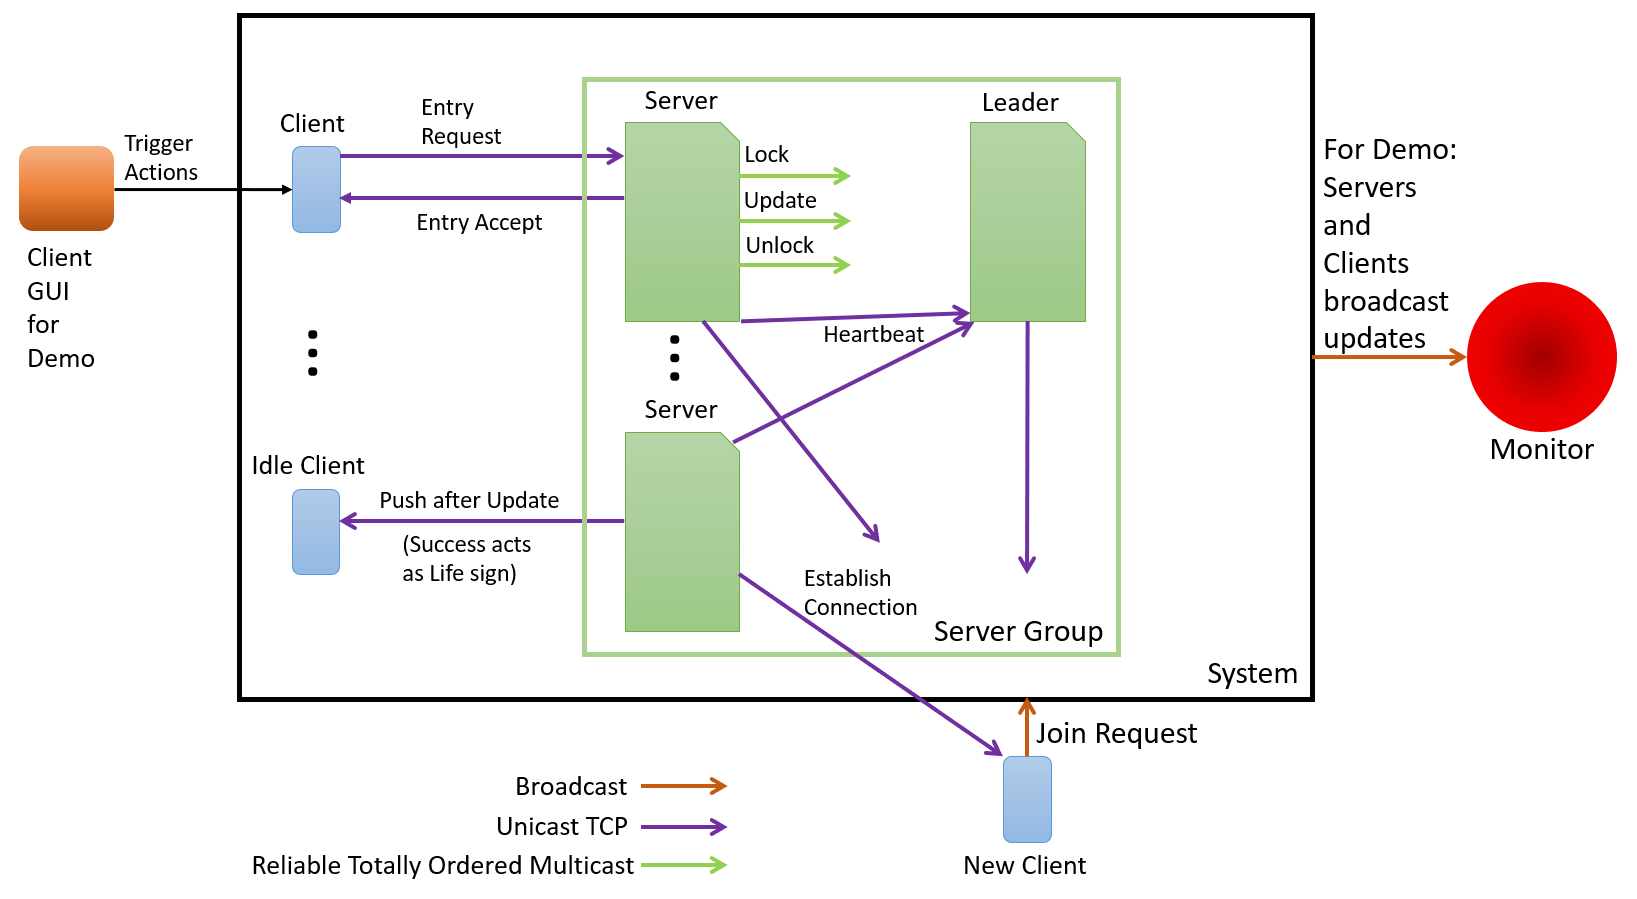
\includegraphics[width=\textwidth]{Architecture_Diagram_new.png}
\end{figure}
\subsection{Demo Setup}
For the demo, we will run several servers and clients on 2+ laptops to ensure a realistic scenario.
Additionally, we implemented both a simple GUI wrapper that can interact with a single client, as well as a demo observer that summarizes the current state of the system.
\section{Implementation Details}
We decided to complete the project using purely Python.
\documentclass[runningheads]{llncs}

\begin{document}

\section{Group Management} \label{grpmngmnt}

The current group view is handled and kept up to date by the leader. Group view updates occur in the following cases:
\begin{itemize}
    \item a member joins the group
    \item a member shuts down intentionally and notifies the leader
    \item  a member fails to send a heartbeat to the leader for two intervals in a row.
\end{itemize}
Any changes on the group view trigger the leader to distribute the group view to all members of the group via TCP.

\subsection{Heartbeats} \label{heartbeats}

Heartbeats are used to monitor the status of the members of the group view. They are used in a bilateral fashion, meaning that the leader checks for failed members as well as members checking that the leader is still operational.

Heartbeats are sent out by each member of the group to the leader via TCP. This action is performed by a threaded timer. Should the leader have shut down or crashed without notifying the group, the TCP connection will fail and the members of the group will trigger a new election. Parallel to this, the leader performs checks on the heartbeat dictionary it maintains. Also triggered by a threaded timer, the leader will check all registered group members and calculate the time difference between the current time and the latest heartbeat it has received from this member.

Should a group member have failed to send a heartbeat for two intervals in a row, it is marked as failed and removed from the group view. Alternatively, if a heartbeat is received by a server that is not/ no longer in the group view, it will be notified and subsequently trigger a new registration process. If a heartbeat is received by a server that is not the leader, an election is triggered.

\end{document}

\documentclass[runningheads]{llncs}
\usepackage{xr}
\usepackage{color}
\externaldocument{group_management}

\begin{document}

\subsection{Voting (Leader Election)}

A leader election can be triggered by three scenarios.

The first scenario is the leader deciding to trigger an election when a new server joins the group and the leader deems it necessary. The necessity of an election is decided based on the group view including the new member. Should the leader no longer fulfill the requirement (largest \textit{uuid}) an election is deemed necessary.

The second scenario is a group member (not leader) not being able to connect to the leader when sending its heartbeat and thus triggering an election. This covers the case that should a leader shut down or crash unexpectedly, the members will pick up on this and trigger an election.

The third scenario occurs when a leader shuts down and broadcasts its shutdown message. Any group member receiving this message will trigger a new election. This should be the standard case in which a leader shuts down planned and properly.

\subsubsection{Election Algorithm}

The implemented algorithm used for leader election is the LCR algorithm. The ring structure allows for easy failure detection in a participating group member as connections between neighbors are established using TCP. Should a group member not be reachable, a new election is triggered. All members have access to and define their next neighbor based on the current group view (see \ref{grpmngmnt}) which leads to an optimal complexity of O(n log n). Should a member find itself to be its own next available neighbor, it will mark itself as the leader, as this implies there are no other available members.

On completion of the leader election, the previous leader will switch its status to \textit{MEMBER} and start sending out heartbeats to the new leader (see \ref{heartbeats}). Accordingly, the new leader will switch its mode to \textit{LEADER} and start listening for heartbeats.

\subsubsection{Failure Management}

Should a node not be able to forward its election message to its next neighbor (as defined by the ring topology), it will remove this neighbor from its own group view and start a new election. To ensure the integrity of the group view, the newly elected leader distributes the group view to all members upon terminating the election algorithm. Before doing so, it cycles through all servers contained in the group view and pings them to ensure they are available. Should a server not be available, it is removed from the group view prior to distribution.

If a node that has declared itself leader crashes before it can abort the election on receiving its own leader message, a subsequent node will receive a leader message without itself being marked as \textit{PARTICIPATING}. In this case, the node will abort the current election and start a new one.

A leader, that has for some reason not participated in the election, but is online at the time the new leader pings the current group, will no longer receive heartbeats from the members of the group, meaning that there are two leaders simultaneously. This case is handled in the process described in \ref{rogueleader}.

\end{document}

\documentclass[runningheads]{llncs}

\begin{document}

\section{Reliable Totally Ordered Multicast} \label{multicast}

Application messages inside the group will be sent via reliable totally ordered
Multicast. In the following, we will describe our implementation and explain
how we handled some corner cases we stumbled across.

\subsection{Procedure} \label{multicastprocedure}

Reliable Totally Ordered Multicast is build upon the IP/Multicast protocol.
Each server has two sockets to realize it, one listener socket which listens on
our defined Multicast address and another socket which is used to send messages
so all messages has a unique sender address. The second socket is needed, so we
know exactly the address who sent a message, so we can answer this server
directly.

If one server sends a message to the group, we add multiple things to the
messages. First we need to give the message a type, so we can distinguish
between messages that are content and messages that are needed for the
protocol. We also add a unique identifier for this message, the unique
identifier of the sender and $S$ of the server. $S$ is needed for reliability
so we know which messages a server missed, so these can be requested for
redelivery.

If the new message was sent, each server listening on the broadcast address,
might now receive this message. First we check if we already received this
message, by comparing the unique message identifier with our received messages.
If we already received the message we can ignore it, if we haven't received it
we put it in our received backlog, and we send a copy of the message to the
group if we aren't the sender of this message. Then we check the piggyback $S$
value and compare it with the current $R$ for that sender. If $S = R + 1$ then
the new message is the next message from this sender, if the $S \leq R + 1$
then the message was already delivered, and we can ignore it and if $S > R + 1$
that means we have missed messages that we either need to request from this
address or messages that could be found in the holdback queue of the server.

We first look at the case where the next message was delivered ($S = R + 1$).
In this case, we then decided to implement ISIS total ordering.
% TODO: Maybe we need to explain here why we need total ordering. Maybe we also
% do this earlier
First we need to set $R$ to $R + 1$, and then we start processing our message
by looking at the type of the message. If the message is a new Application
message we need to propose an order to the original sender by answering with a
$pq = max(aq, pq) + 1$. $aq$ is the largest agreed sequence number and $pq$ is
the largest proposed sequence number. This message will be sent to the second
socket address, not via Multicast, so it only reaches the server which needs
the answers.

This server will then collect these answers from all active members in the
group (we will discuss later how we are handling this with dynamic joining and
leaving servers \ref{multicastchanges}). When all messages are collected the
server will broadcast a new message, with a different type. The content of the
message is the agreed sequence number $a =
max(all\_proposed\_sequence\_numbers)$. We also add a unique ID, sender ID and
the next $S$ to this message, so the message is also reliable.

Upon receiving the message, we compare the $S$ value with the current $R$ the
same way as described above, but we handle the message a different if $S = R +
1$. Now we need to reorder the delivery group based on the received $a$. The
delivery queue is the queue of the next messages that will be delivered, we
have two queues to make it easier for us to handle. A holdback queue of
messages that can't be processed yet because of missing messages and the
delivery queue.

Now we look into what we can do if we notice that we have missed a message. If
$S > R + 1$ we know we have missed at least one message from the sender. We put
this new message in our holdback queue, for later processing and then look
inside the whole back queue if we maybe already received the next message in
the order defined by $S$ and $R$. If that is the case, we process these
messages and remove them from the holdback queue until we find a message for
that $S = R + 1$ is no longer true. We collect all missing $S$ numbers and send
the server a 1 to 1 message that we are missing these $S$ numbers. The server
will then collect these messages and resend them. Both messages aren't
protected with an S because if the message is lost, we run into the next
failure of $S = R + 1$ when the next broadcast message arrives, and we end up
running the algorithm again.

\subsection{Server leaving and joining the group} \label{multicastchanges}

If a new server joins, the group management will make sure that all servers set
up the new member correctly and set $R$ for this server to 0. When the leader
welcomes the new server, it also shares his current $R$ numbers of all the
members of the group and all messages in the delivery queue, so that the new
server can handle a next message that might be an order proposal.

When waiting for proposal messages, the server will not wait for a proposal
from the new joined server, if the server wasn't active when the original
messages was sent. We realize this by keeping a snapshot of the group view at
the time the message was sent. We then only wait for messages of members from
$members_at_time_of_sending \cap current_members$. This also solves the issues
that we no longer wait for messages from server, which already left the group.

\end{document}


\documentclass[runningheads]{llncs}

\begin{document}

\subsection{Byzantine Fault Tolerance} \label{byzantine}

To support fault tolerance, we decided to implement the byzantine algorithm. In
the following, we will describe our implementation and explain how we handled
some corner cases we stumbled across.

\subsubsection{Procedure} \label{byzantineprocedure}

Byzantine algorithm is a synchronous message based algorithm which is used to
implement a form of fault tolerance. To implement this synchronous algorithm in
our asynchronous distributed system we decided to move the system in a state
where we can run this algorithm. For this, we need to pause every application
specific reliable totally ordered multicast~\ref{multicast} message until the
algorithm is completed. This state change is initiated by the leader when a new
server joins. If the system has 4 or more servers, the minimum amount of
servers required for byzantine, the leader sends a pause multicast message via
multicast to all participants in the system. This means that each server pauses
application messages over reliable totally ordered multicast by putting them in
a queue, but not sending them. This allows us to still send internal messages
over reliable totally ordered multicast, for example the resume message. Once
the algorithm is completed, the leader sends a resume multicast message which
means that servers are again permitted to send out multicast messages. So the
queue that hold all application messages, that were not sent out yet will be
emptied.

When all servers are paused, the leader initiates the byzantine algorithm by
sending the byzantine message, named in the following $OM$ to all servers in
the group. The message consists of a $v$ which we chose as the current entries
(application data) on each server, the server destinations, which are all
servers in the group without the leader server, the list of servers which are
passed, on initiation, only the leader, and a $f = \lfloor (n - 1)/ 3 \rfloor$.
This message will be sent to all destinations, as previously defined, via tcp.

On receiving of this message, each server will start a new tree, if not already
started, where it keeps track of all received $OM$ messages. It removes itself
from the list of destinations, adds himself to the beginning of the list of
passed servers, does $f = f - 1$, adds his own entries count as $v$ and packs
everything in a new message $OM'$ which will be sent to all servers left in the
destination list.

This repeats until all messages are sent, and we end up with a tree on each
server that is not the leader. We are then calculating the most common value
for each level, starting at $f - 1$ and for node and select the most common one
out of this list. This most common element will be sent back to the leader
which will then select the most common element from all answers and distribute
the result, with a resume multicast over reliable totally ordered multicast to
all servers. Every server will then take the result as the new value for the
current entries.

If a TCP-Message is not being delivered, we can assume that the connection to
this server is lost and that the group view might have changed. Because of this
we decided to restart the byzantine algorithm if there are still enough server
in the group. This is done by sending a restart message to the current leader
which will then start a new run with a new unique ID. Making the old one
invalid. So if a server receives a byzantine message with a new ID that he
doesn't know he has to discard the current tree and start a new one.

If a new Server wants to join the group while byzantine is running, the leader
answers with a wait for message that signals the new server that there is a
group, but it is not yet permitted to join. The leader will then memorize that
a new server wants to join and will accept that server as soon as the byzantine
algorithm is done.

\end{document}


\documentclass[runningheads]{llncs}

\begin{document}
\subsection{Client}

\end{document}

\documentclass[runningheads]{llncs}

\begin{document}

\subsection{Monitoring and GUIs}

\subsubsection{System Monitor}
Monitoring on a per-node basis is implemented in the form of logging, utilizing log-levels to control the verbosity. A monitoring-server with a simple graphical user interface provides a global overview of the current state of the servers in the system. Various parameters such as server-UID, currently connected clients, election participation state, byzantine participation state and server state (\textit{LEADED, MEMBER, PENDING}) are displayed. The monitoring server has no direct interaction with the system as it utilizes UDP to listen for specific monitoring data which the individual servers are promoting. To reduce the number of messages being sent on the network, data is only promoted based on events and at regular intervals, namely when a server sends its heartbeat.

\subsubsection{Client GUI}
A basic client interface is implemented for simplified interaction and to demonstrate the intended application of the system. It displays the currently connected server, a count of visitors within the venue and two buttons for interaction: one for a visitor entering the venue and one for a visitor leaving. Upon requesting entry, visual feedback is provided in the case of a confirmation or denial.

\end{document}
\newpage
\section{Code}
We will have sent invitations to our private code repository on github by the time this report is read.

\section{Discussion and Conclusion}
Working on this project made clear that even a very simple application requires a large amount of effort before it can be safely run in a distributed way, despite the aspect of security being ignored.
\\\\
From basic functionality to algorithms used for voting, finding a consensus and ensuring data integrity, additional considerations had to be made for cases such as members or message-recipients becoming unreachable mid-process. Which of these issues to handle had how to handle them had to be made based on severeness of impact on the system, as covering all of them would have not been possible in the given time.
Frequently, new edge cases would be found during tests and dealt with  before making sure to reproduce them correctly during later tests to ensure they had been fixed.
Additionally, locating a fault often proved more complex than when dealing with a local or monolithic system, often requiring to log all messages received by the different system components and backtrack to exactly what went wrong in the first place.

Future considerations would include finding an alternate solution to using heartbeats. As the group view relies heavily on (missed) heart beats, it can take a noticeable amount of time for the system to update depending on the heartbeat-interval.
This also means that at times, multicast messaging stalls until the system is sorted out again. The system is eventually-consistent, nevertheless, how well suited this is for a real-time application is debatable.
Additionally, tests with eight or more servers clearly showed the limitations of the byzantine algorithm, as its exponential message complexity flooded the channel, also stalling the system.
In general, not much consideration was given to message complexity, as it was not the objective of this project. However, it did show the importance of complexity and efficient algorithms within such a system, as the above implementation quickly brought our consumer-grade hardware to a sweat.
\\\\
All in all, the experience gained from this project should help in making better decisions not only when developing system components actually concerned with distribution, but also when developing components that will run in a distributed system and should thus be ready to deal with faults not present in a monolithic system.
\end{document}
